\chapter{Realisierung}
\section{Modellierung}
Blenderplugin, IFCWallTypes Module die das Raster vorgeben etc.

\section{Wall Detailing}
In Abschnitt~\ref{concept:wall_detailing} wurde das Wall Detailing als der Vorgang, ein als geometrischer Körper definiertes Wandstück in ein konkretes Mauerwerk zu überführen, bezeichnet.
Innerhalb des IFC Standards werden einige mathematische/geometrische Repräsentationen der sogennanten \textit{IFCWall} unterstützt, um neben einfachen Boxen auch komplexere Formen abbilden zu können.
Beispielsweise ist es möglich in das Modell eines Hauses zunehmend dünner werdende Wandstücke, kurvige Wandstücke oder Wandstücke, welche nur durch ein arbiträres Vieleck beschrieben werden können zu integrieren.
Allerdings ist es für die Fallstudien dieser Arbeit zunächst ausreichend lediglich Wandstücke, welche als einfacher geometrischer Quader vorliegen, zu beachten.
Das nachfolgende schrittweise Vorgehen weist aufgrund des annähernd gleichen Ergebnisses zwangsläufig Ähnlichkeiten zu dem von Usmanov et al. auf \cite{Usmanov2021}.

\subsection{Konvertieren des IFC zu BREP}
Den ersten Schritt stellt das Extrahieren aller notwendigen Daten aus dem vorliegenden IFC Modell dar.
Für die Fallstudien dieser Arbeit sind sowohl alle Objekte des Typs \textit{IFCWall} als auch die, etwa durch Fenster oder Türen entstehenden, daran angeknüpften Objekte vom Typ \textit{IfcOpeningElement} (siehe \ref{basics:IfcOpeningElement}) von Interesse.
Zusätzlich werden aus den, in den \textit{IfcPropertySets} der Wandstücke hinterlegten Daten, Informationen über das zu verwendende Modul ausgelesen.
Mithilfe der Werkzeuge der in Kapitel \ref{basics} vorgstellten Python Bibliothek \textit{ifcopenshell} (siehe \ref{basics:ifcopenshell}) ist dies intuitiv möglich.
TODO Sätze zum Code, Code TODO kleines Klassendiagram von Wall/WallLayerGroup und Opening und BrickInformation

\subsection{Überprüfen der modellierten Wände}
\subsubsection{Filtern}
Da sich diese Arbeit zunächst ausschließlich mit quaderförmigen Wandstücken beschäftigt, müssen zunächst alle zuvor aus dem IFC Modell extrahierten Wandstücke auf diese Eigenschaft geprüft werden.
Somit ist gewährleistet, dass lediglich passende Wandstücke an die nachfolgenden Schritte weitergegeben werden.
TODO Satz zum Code, Code iscubic

\subsubsection{Anwenden des Moduls}
Mit dem zu jedem Wandstück festgelegten Modul werden nun alle Wandstücke in Schichten aufgeteilt.
Deren Höhe entspricht im Normalfall der Höhe des jeweilgen Moduls.
Lediglich die oberste Schicht kann durch falsch modellierte Wandstücke eine niedrigere Schichthöhe aufweisen.
Dies ist der Fall, wenn die Gesamthöhe des Wandstücks nicht exakt einem Vielfachen der Höhe des Moduls entspricht und ein nicht aufzuteilender Rest existiert.
Das Aufteilen in Schichten erleichtert es im Anschluss Berechnungen an Wandstücken durchzuführen und Beziehungen zwischen ihnen zu finden.

\subsubsection{Kombinieren passender Wandstücke}
\label{real:combination}
Eine solche Beziehung stellen Wände dar, die, wie bereits in Kapitel~\ref{concept:relations_wandtuecke} definiert, durch mehrere einzelne Objekte modelliert wurden, eigentlich aber eine Einheit bilden.
Daher werden in diesem Schritt alle Wandstücke miteinander verglichen und eventuell kombiniert, sodass jeweils ein gefundes Paar durch ein einzelnes Wandstück representiert wird.
Um zwei Wandstücke zu sinvoll kombinieren zu können, müssen die Eigenschaften aus Kapitel~\ref{concept:combination_properties} gelten.
Allerdings kann Punkt~\ref{concept:schichten}, welcher Berührung oder Überlappung voraussetzt mittlerweile wie folgt verschärft werden:

\begin{enumerate}
\setcounter{enumi}{4}
\item\label{real:schichten} Mindestens eine Schicht des einen Wandstücks berührt, überlappt oder befindet sich exakt eine Modulöhe ober- oder unterhalb einer Schicht des anderen Wandstücks.
\end{enumerate}

In Abbildung~\ref{fig:concept:combination_example_base} treten verschiedene Konstellationen von Wandstücken auf, die miteinander kombiniert werden müssen.
Das aus Wandstück 1 und 2 gebildete Paar erfüllt alle oben genannten Eigenschaften und weist eine Teil-Überlappung auf.
Somit müssen beide Wandstücke miteinader kombiniert werden.
Den obersten Bereich füllen sowohl Wandstück 5 als auch Wandstück 6, sodass dort eine komplette Überlappung vorliegt.
Auch diese beiden Wandstücke werden kombiniert, wobei dabei im Prinzip einfach eines verworfen wird.
Zusätzlich muss dieser Bereich, wie auch Wandstück 7, mit Wandstück 2 kombiniert werden, da die beiden Paare sich an Ober- und Unterkante berühren.
Einen weiteren Fall stellen seitliche, nicht überlappende Berührungen dar, wie sie zwischen Wandstück 2 und 3 zu sehen ist.
Auch für dieses Paar sind alle Voraussetzungen zur Fusion erfüllt.
Lediglich Wandstück 4 muss nicht mit dem Rest vereint werden, da dafür kein Paar existiert, das die obrigen Eigenschaften erfüllt.
Anhand von Abbildung~\ref{fig:real:combination_example_solution_xoffset} kann man erkennen, dass Wandstück 4 im weiteren Verlauf des Detailings tatsächlich unabhängig betrachtet werden kann. 

Während dem Kombinieren von zwei Wänden, wird ein Wandstück schichtweise in das andere überführt.
Dabei werden alle Schichten paarweise miteinader verglichen, um diejenigen Paare zu finden, die die Eigenschaften aus Punkt~\ref{real:schichten} erfüllen.
Ein solches Paar wird dann wie folgt miteinander verschmolzen:

\begin{lstlisting}[language=Python, caption=Pseudocode zur Vereinigung zweier sich berührender oder überlappender Schichten von zwei nach den Voraussetzungen aus Abschnitt~\ref{concept:combination_properties} kombinierbaren Wandstücken.]
  def combine(layer1, layer2):
    # get the local positions of both edges of layer1 as 3D array
    left_edge1 = layer1.get_left_edge(relative=True)
    right_edge1 = layer1.get_right_edge(relative=True)

    # get the position of both edge of layer 2 relative to the coordinate systsem of layer1 as 3D array
    left_edge2 = layer2.get_left_edge(relative=False)
    left_edge2 = layer1.relative_position_of(left_edge2)

    right_edge2 = layer2.get_right_edge(relative=False)
    right_edge2 = layer1.relative_position_of(righ_edge2)

    # get the total length both layers cover by subtracting max - min of the x coordinates
    max_x = max(left_edge1[0], right_edge1[0], left_edge2[0], right_edge2[0]) 
    min_x = min(left_edge1[0], right_edge1[0], left_edge2[0], right_edge2[0]) 
    total_length = max_x - min_x

    # calculate the center of the resulting layer
    left = min([a1, a2, b1, b2], key=lambda x: x[0])
    local_center = left.copy()
    local_center[0] += total_length / 2.0

    # convert to global coordinates and return new layer
    center = layer1.global_position_of(local_center)
    return Layer(center, total_length)

\end{lstlisting}

TODO erklärung Code

\begin{figure}[ht!]
  \centering
  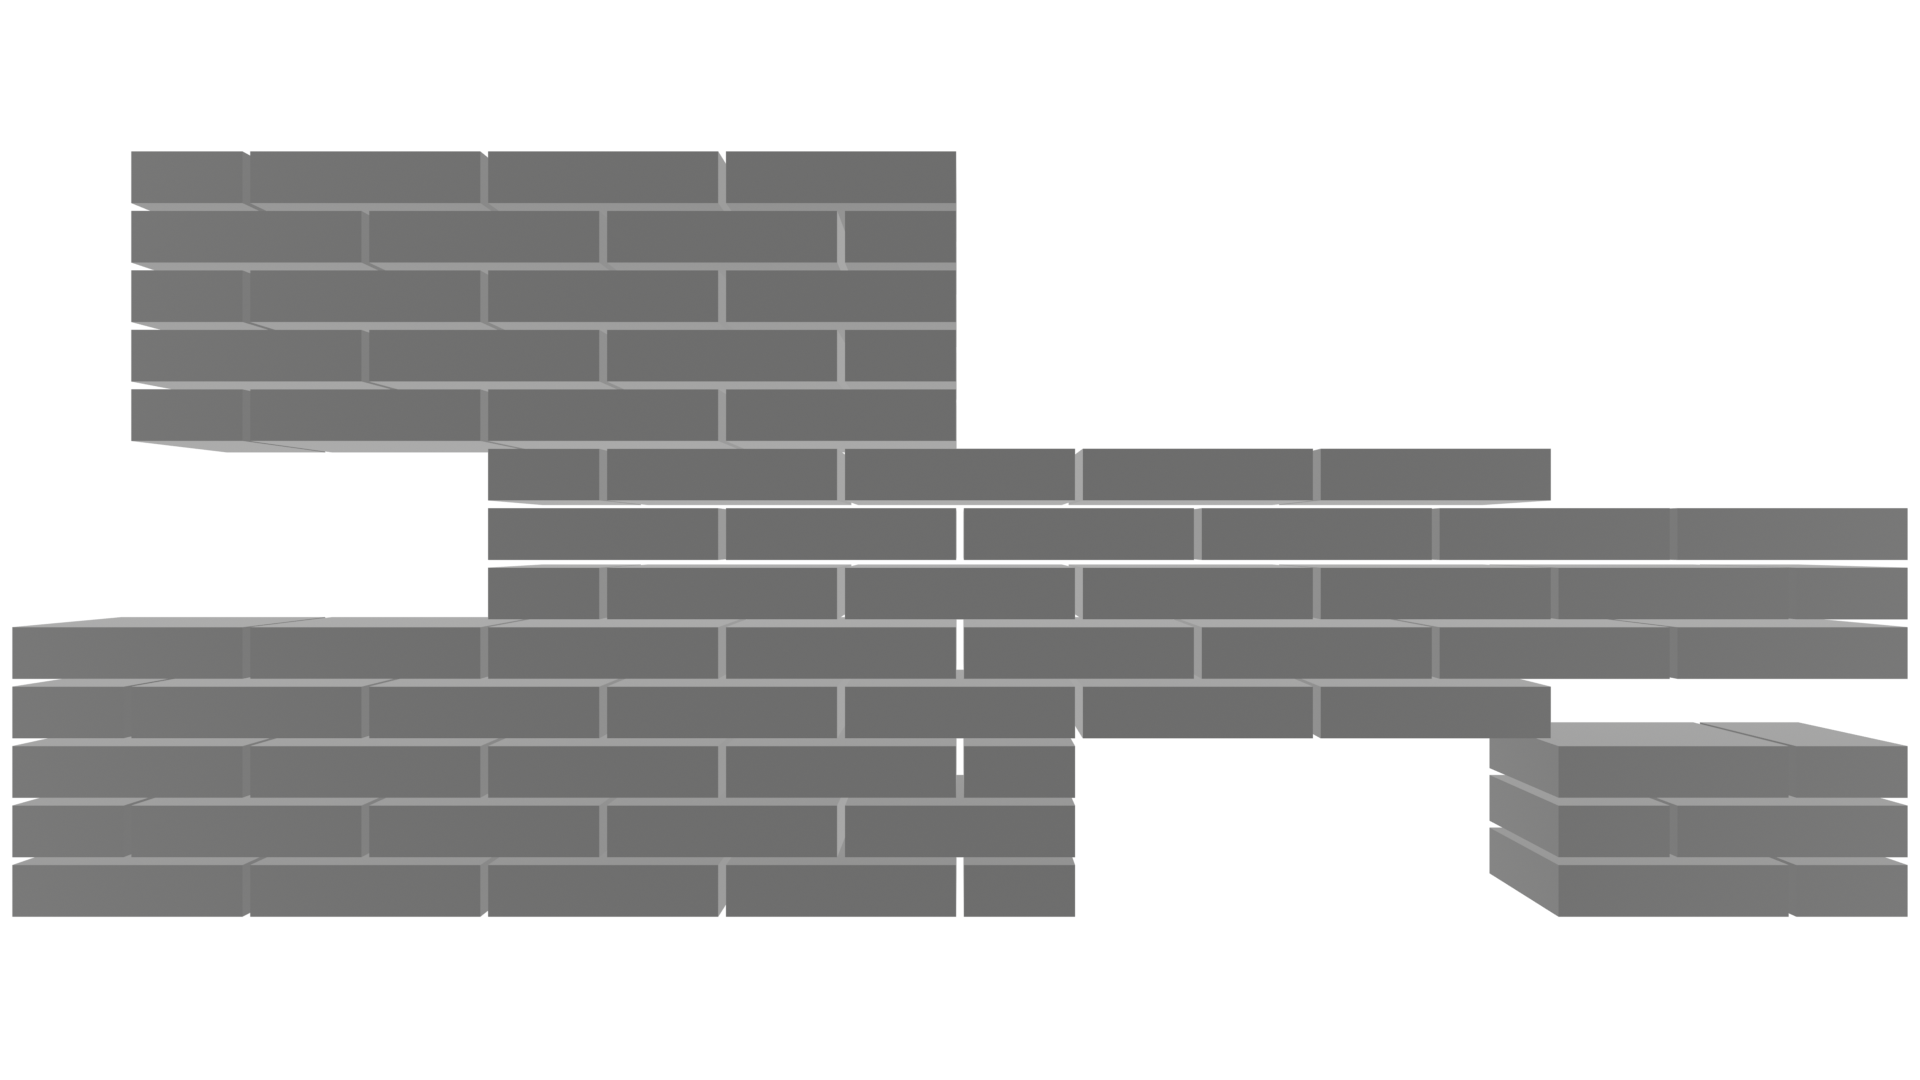
\includegraphics[width=0.8\columnwidth]{fig/Real_Combination_Output.png}
  \caption{Ergebnis mit berücksichtigtem \textit{x\_offset}.}
  \label{fig:real:combination_example_solution_xoffset}
\end{figure}

\begin{figure}[hb!]
  \centering
  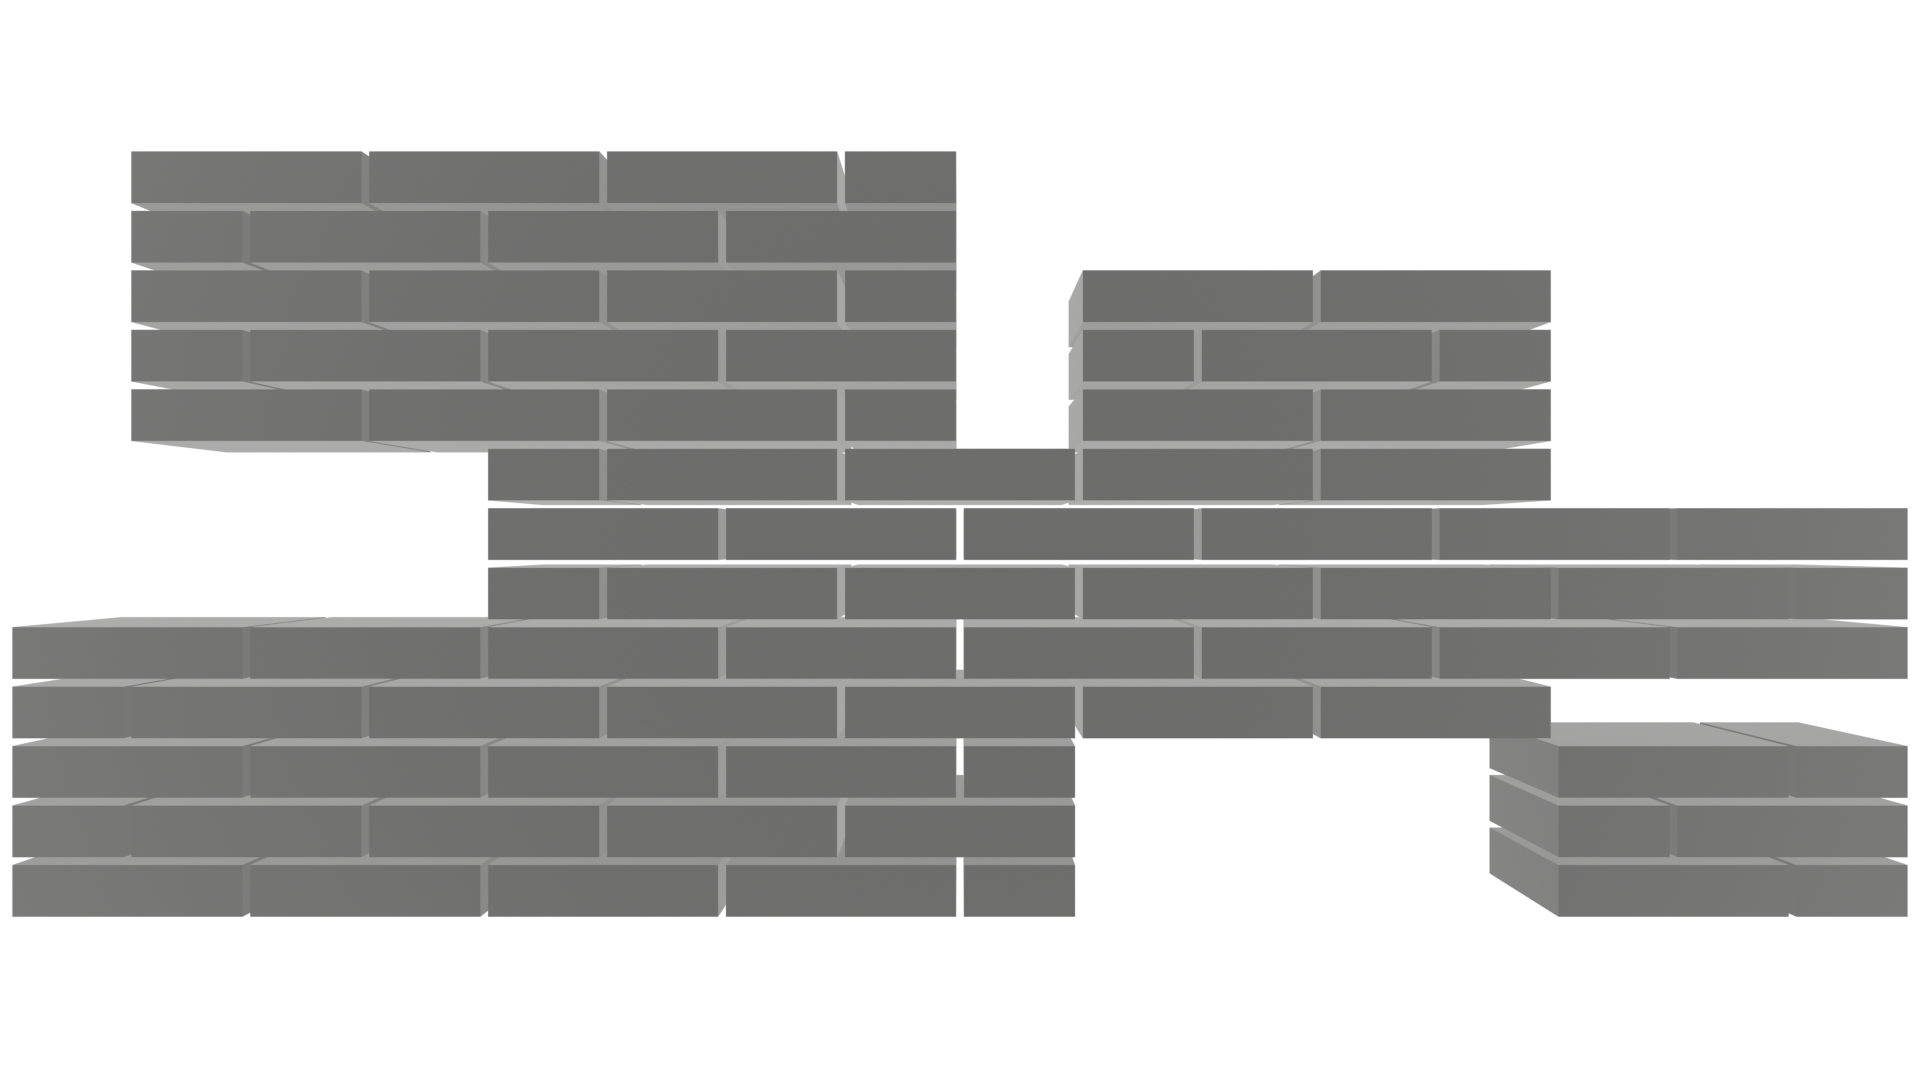
\includegraphics[width=0.8\columnwidth]{fig/Real_Combination_Output_No_XOffsetpng.png}
  \caption{Ergebnis mit ignoriertem \textit{x\_offset}.}
  \label{fig:real:combination_example_solution_no_xoffset}
\end{figure}

Steht ein Wandstück in X-Richtung versetzt auf einem anderem, so ist es notwendig diesen Versatz während dem nachfolgenden Detailing zu berücksichtigen.
Ignoriert man dies, kann das zu den in Abbildung~\ref{fig:real:combination_example_solution_no_xoffset} gezeigten Fehlern (zum Beispiel zwischen Wandstück 2 und 7) innerhalb des Mauerwerksverbands und damit ebenfalls zu Verletzungen des vorgeschriebenen Überbindemaßes führen (siehe Abschnitt~\ref*{basics:Mauerwerksverband}).
Dieser, nachfolgend als \textit{x\_offset} bezeichnete Versatz ist definiert durch die Differenz zwischen der kleinsten lokalen X-Koordinate aller Schichten eines Wandstückes und der lokalen X-Koordinate der zu betrachtenden Schicht.
Der daraus resultierende Wert wird später dazu verwendet den anzuwendenden Mauerwerksverband erst an der passenden Stelle zu beginnen.
Dadurch erzielt man einen einheitlichen Verband über das gesamte Wandstück und verhindert den in Abbildung~\ref{fig:real:combination_example_solution_no_xoffset} gezeigten Fehlerfall.
Eine weitere Eigenschaft, die aus dem Kombinieren mehrerer Wandstücke entstehen kann, ist das vorhandensein unterbrochender Schichten oder, anders ausgedrückt, mehrerer Schichten auf einer Höhe innerhalb des resultierenden Wandstückes.
Dies ist ebenfalls in Abbildung~\ref{fig:real:combination_example_base} zu sehen. 
Zwischen drei Schichten des Bereichs der Wandstücke 5 und 6 und des Wandstücks 7 ist eine Lücke.
Durch das Einbeziehen des \textit{x\_offset} können derartige Situationen jedoch ebenfalls gelöst werden, da für jedes Teilstück einer Schicht ein eigener \textit{x\_offset} berechnet wird.

Nach Vereinigung aller passenden Paare reduziert sich die Zahl der ursprünglichen Wandstücke aus dem Modell in Abbildung~\ref{fig:concept:combination_example_base} von 7 auf 2.

\subsubsection{Beziehungen finden}
Nun wird die aus dem vorherigen Schritt entstandene neue Menge an Wandstücken auf weitere Beziehungen untersucht.
Für das Wall Detailing relevante Beziehungen stellen Ecken, T-Kreuzungen und X-Kreuzungen dar (siehe \ref{basics:Mauerwerksverband}).
Der Grund dafür ist die Komplexität in diesen Bereichnen die vorgeschriebenen Normen (wie etwa dem in Abschnitt~\ref{basics:Mauerwerksverband} genannten Überbindemaß) einzuhalten.
Deswegen existieren für jeden Mauerwerksverband eigene spezielle Eck- und Kreuzungslegepläne, die an diesen Stellen eingefügt werden müssen.
Es werden wie oben nur die Wandstücke miteinander verglichen, die mit dem selben Wandtyp annotiert wurden und das gleiche Modul verwenden.
Da die drei Beziehungen sich stark ähneln, besitzen sie einige geteilte Eigenschaften:
\begin{enumerate}
    \item Die lokalen Z-Achsen beider Wandstücke sind parallel. Das Vorgehen zur Überprüfung ist dasselbe wie in Abschnitt~\ref{real:combination}.
    \item Sie stehen auf der selben Höhe oder versetzt um ein Vielfaches der gemeinsamen Modulhöhe.
    \item Mindestens eines der beiden Wandstücke endet auf einem anderen, sodass mindestens eine Schicht das andere Wandstück direkt berührt.
\end{enumerate}
Sind diese Eigenschaften erfüllt, werden für jede durch die einzelnen Schichten der Wandstücke vorgegebene Höhe Schnittpunkte zwischen den beiden Wandstücken errechnet.
Im Falle einer einfachen Ecke oder einer T-Kreuzung, existiert nur ein einzelnes Paar an Wandstücken, deren Schichten sich in jedem Höhenschritt des Moduls im Mittelpunkt der Ecke schneiden.
Der Unterschied ist lediglich die Stelle des Schnittpunkts relativ zu den beiden Wandstücken.
Liegt der errechnete Schnittpunkt bei beiden Wandstücken näher als Wandbreite/2 an einer der beiden Außenkanten handelt es sich um eine Ecke.
Falls der Schnittpunkt bei einem der beiden Wandstücke allerdings mindestens Wandbreite/2 innerhalb des Wandstücks liegt, so handelt es sich um eine T-Kreuzung.
Werden für zwei unterschiedliche Paare die selben Schnittpunkte errechnet, so kann es sich entweder um eine mit drei Wandstücken modellierte T-Kreuzung oder X-Kreuzung handeln.
Teilen sich zwei T-Kreuzungen die selben Schnittpunkte, so sind alle Vorraussetzungen für eine eine X-Kreuzung gegeben.
Liegt der Schnittpunkt des Wandstück-Paares mindesten Wandbreite/2 innerhalb beider Wandstücke, so handelt es sich um eine X-Kreuzung - modelliert aus zwei sich schneidenden Wandstücken. 
TODO Bilder

\subsection{Lösen der Beziehungen}
Je nach gewählten Verband müssen z.B. Ecken (deren Baupläne im vornherein definiert wurden) so angeordnet werden, dass die dazwischenliegenden Wandstücke lückenlos eingefüllt werden können.
Dafür muss ein sogenannter "plan\_offset" für jede Wand und jede Ecke gefunden werden. Dieser gibt an, an welchem Index der Bauplandefinition das Wandstück (von unten) beginnen muss, um insgesamt einen einheitlichen Wandkörper ohne Lücken zu bilden.
Voraussetzung dafür ist natürlich ein passender Eckplan zu dem gewählten Verband. 

Schwierigkeiten: Eckpläne insgesamt, Ecken ragen in die sie bildenden Wände hinein. Diese müssen dementsprechend verkleinert werden.

\subsection{Anwenden der Lösung}
Ablaufen aller Ecken und Wände und einsetzen der Ziegel gemäß den gefundenen Lösungen.

\subsection{Export}
Abhängigkeitsgraph und Ontologie für Regelwerk